\chapter{Primeiro Experimento}
\label{chap:primeiro_experimento}

%! Escrever um pouco sobre o que foi feito

Utilizando a técnica de \ac{DOE}, descrita no Capítulo \ref{chap:descricao_do_experimento}, pode-se gerar um conjunto de casos teste para todas as possíveis combinações de variações do modelo do helicóptero de papel em estudo. As variações em estudo são a altura de lançamento do helicóptero de papel, a presença do clipe de papel, dos adesivos no topo e nas laterais do modelo.

\section{Criando o experimento no R}
\label{sec:primeiro_experimento_criando o experimento_no_R}

%! Escrever sobre código usado para criar o experimento, a sequencia de testes, no R. Qual o motivo de usar isso?

Com o intuito de gerar esse conjunto de testes de forma a minimizar a inserção de \textit{bias} ou interferência humana nos resultados obtidos, foi desenvolvido um código na linguagem R, disposto no Apêndice \ref{sec:app_codigo_geracao_do_experimento_de_modelagem}, para a criação da lista de experimentos que é apresentada na Tabela \ref{tab:experimento_modelagem_helicoptero_papel}.

\begin{table}[H]
  \centering
  \caption{Experimento de modelagem do helicóptero de papel.}
  \resizebox{0.6\textwidth}{!}{%
  \begin{tabular}{c|c|c|c}
  \textbf{Altura} & \textbf{Clipe} & \textbf{AdesivoTopo} & \textbf{AdesivoLateral} \\ \hline
  1.3             & -              & +                    & +                       \\ \hline
  2.1             & +              & +                    & -                       \\ \hline
  1.3             & -              & -                    & +                       \\ \hline
  2.1             & +              & -                    & -                       \\ \hline
  1.3             & +              & -                    & -                       \\ \hline
  2.1             & -              & +                    & -                       \\ \hline
  2.1             & -              & -                    & -                       \\ \hline
  1.3             & +              & +                    & +                       \\ \hline
  2.1             & -              & -                    & +                       \\ \hline
  1.3             & -              & -                    & -                       \\ \hline
  2.1             & +              & +                    & +                       \\ \hline
  2.1             & +              & -                    & +                       \\ \hline
  2.1             & -              & +                    & +                       \\ \hline
  1.3             & -              & +                    & -                       \\ \hline
  1.3             & +              & -                    & +                       \\ \hline
  1.3             & +              & +                    & -
  \end{tabular}%
  }
  \legend{Fonte: Autores.}
  \label{tab:experimento_modelagem_helicoptero_papel}
\end{table}

\section{A coleta de dados}
\label{sec:primeiro_experimento_a_coleta_de_dados}

%! Escrever sobre como foi feita a coleta de dados e indicar a tabela resultante

Utilizando a sequência de variações do modelo de helicóptero de papel apresentada na Tabela \ref{tab:experimento_modelagem_helicoptero_papel}, foram realizados os experimentos necessários tal como pode ser visto na Figura \ref{fig:primeiro_experimento}. Todos os lançamentos dos helicópteros foram feitos por um dos integrantes da equipe. Por sua vez, as tomadas de tempo foram feitas por outras duas pessoas, sendo o último integrante da equipe responsável pela anotação dos valores obtidos. Os tempos de vôo de cada experimento estão dispostos na Tabela \ref{tab:dados_experimentais_para_modelagem}.

\begin{figure}[H]
  \centering
  \caption{Um dos lançamentos do helicóptero de papel para realização do experimento.}
  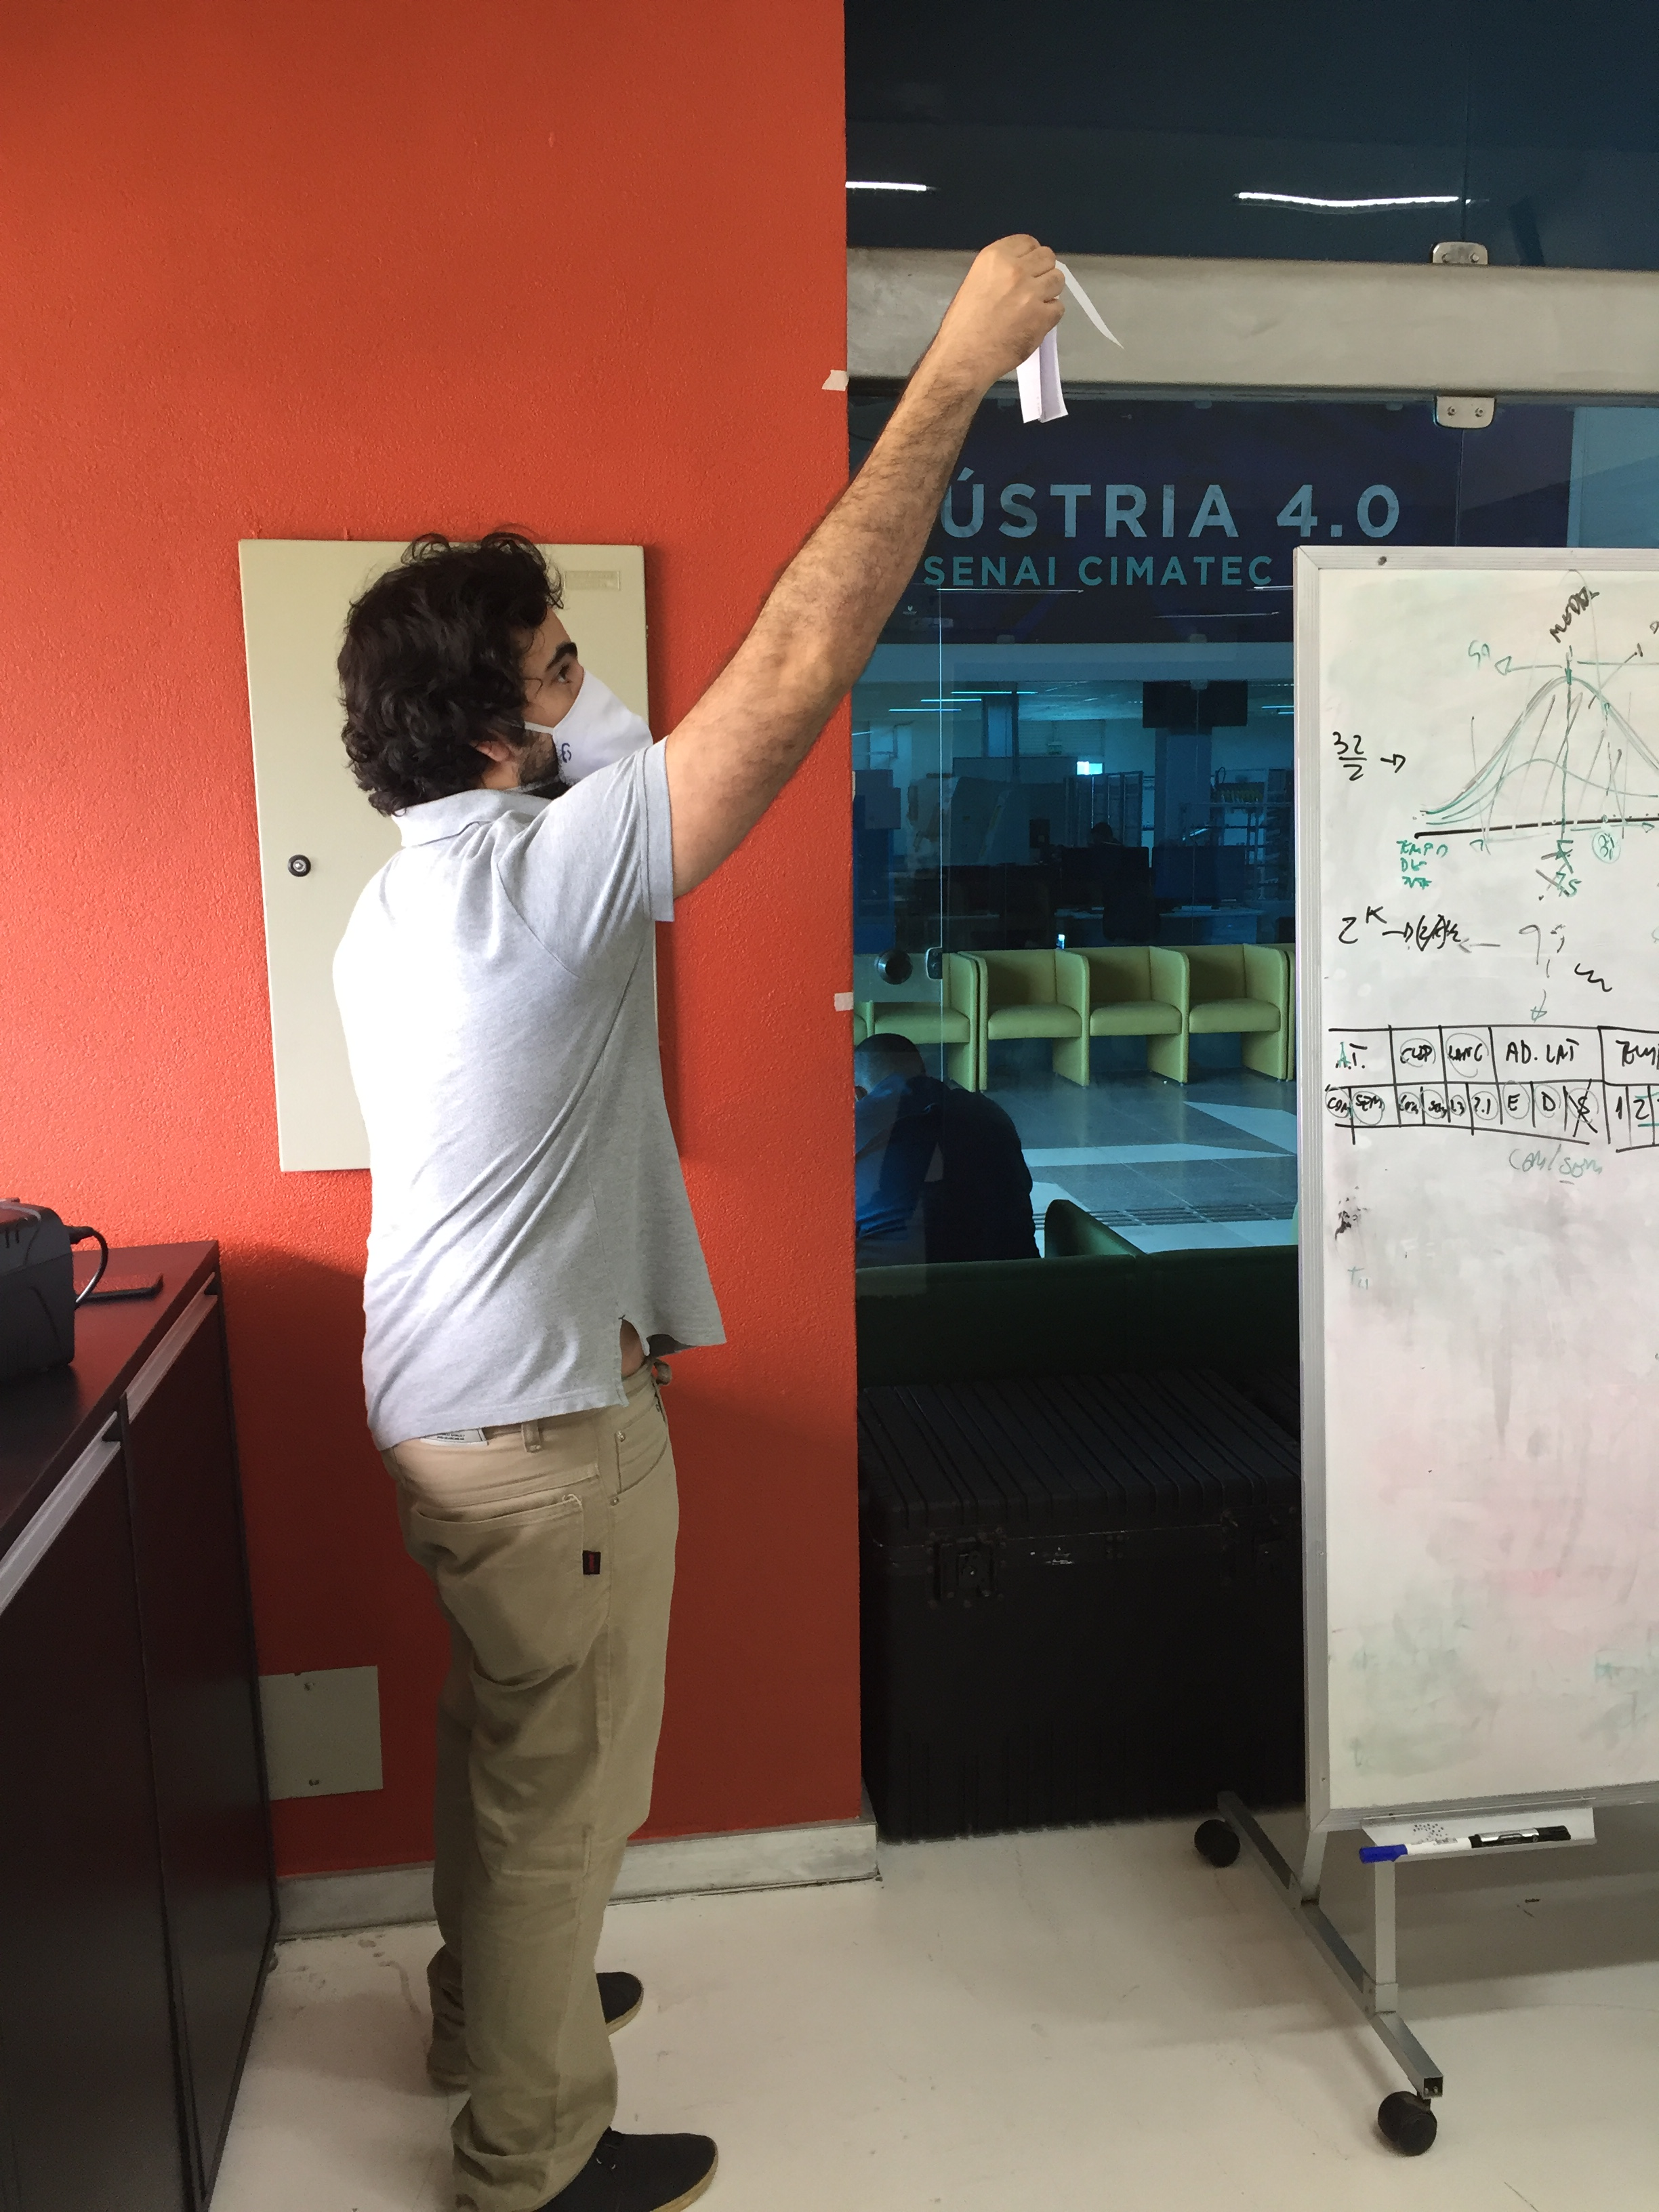
\includegraphics[width=0.8\textwidth]{images/20200909_145557439_iOS.png}
  \legend{Fonte: Autores.}
  \label{fig:primeiro_experimento}
\end{figure}